\section{ITK Introduction}


\centeredlargetext{white}{black}{
ITK Introduction
}

\begin{frame}
\frametitle{ITK is a Templated Library}
You will typically do:
\begin{itemize}
\item Include headers
\pause
\item Pick pixel type
\pause
\item Pick image dimension
\pause
\item Instantiate image type
\pause
\item Instantiate filter type
\pause
\item Create filters
\pause
\item Connect pipeline
\pause
\item Run pipeline
\end{itemize}
\end{frame}

{
\setbeamertemplate{navigation symbols}{}
\begin{frame}[fragile]
\frametitle{Basic Filtering - Median Filter}
\framesubtitle{ITKIntroduction/exercise1/BasicImageFilteringITK.cxx}
\begin{itemize}
\item Include headers
\end{itemize}
\lstlistingwithnumber{19}{21}{BasicImageFilteringITK.cxx}
\pause
\begin{itemize}
\item Read images from files
\item Write images from files
\item Apply a median filter in an image
\end{itemize}
\end{frame}
}

{
\setbeamertemplate{navigation symbols}{}
\begin{frame}[fragile]
\frametitle{Basic Filtering - Median Filter}
\framesubtitle{ITKIntroduction/exercise1/BasicImageFilteringITK.cxx}
\begin{itemize}
\item Declare pixel types and image dimension
\lstlistingwithnumber{32}{35}{BasicImageFilteringITK.cxx}
\end{itemize}
\pause
\begin{itemize}
\item Declare input and output image types
\lstlistingwithnumber{37}{38}{BasicImageFilteringITK.cxx}
\end{itemize}
\end{frame}
}

{
\setbeamertemplate{navigation symbols}{}
\begin{frame}[fragile]
\frametitle{Basic Filtering - Median Filter}
\framesubtitle{ITKIntroduction/exercise1/BasicImageFilteringITK.cxx}
\begin{itemize}
\item Declare the types for reader and writer
\lstlistingwithnumber{40}{41}{BasicImageFilteringITK.cxx}
\end{itemize}
\pause
\begin{itemize}
\item Instantiate the reader and writer objects (source and sink)
\lstlistingwithnumber{43}{44}{BasicImageFilteringITK.cxx}
\end{itemize}
\pause
\begin{itemize}
\item Set input and output filenames
\lstlistingwithnumber{46}{47}{BasicImageFilteringITK.cxx}
\end{itemize}
\end{frame}
}

{
\setbeamertemplate{navigation symbols}{}
\begin{frame}[fragile]
\frametitle{Basic Filtering - Median Filter}
\framesubtitle{ITKIntroduction/exercise1/BasicImageFilteringITK.cxx}
\begin{itemize}
\item Declare the Median filter type
\lstlistingwithnumber{49}{50}{BasicImageFilteringITK.cxx}
\end{itemize}
\pause
\begin{itemize}
\item Create the filter
\lstlistingwithnumber{51}{51}{BasicImageFilteringITK.cxx}
\end{itemize}
\end{frame}
}

{
\setbeamertemplate{navigation symbols}{}
\begin{frame}[fragile]
\frametitle{Basic Filtering - Median Filter}
\framesubtitle{ITKIntroduction/exercise1/BasicImageFilteringITK.cxx}
\begin{itemize}
\item Define the Median kernel radius (Manhattan Radius)
\lstlistingwithnumber{55}{58}{BasicImageFilteringITK.cxx}
\end{itemize}
\pause
\begin{itemize}
\item Connect the pipeline
\lstlistingwithnumber{60}{61}{BasicImageFilteringITK.cxx}
\end{itemize}
\end{frame}
}

{
\setbeamertemplate{navigation symbols}{}
\begin{frame}[fragile]
\frametitle{Basic Filtering - Median Filter}
\framesubtitle{ITKIntroduction/exercise1/BasicImageFilteringITK.cxx}
\begin{itemize}
\item Trigger the pipeline execution by calling Update().
\lstlistingwithnumber{63}{71}{BasicImageFilteringITK.cxx}
\end{itemize}
\pause
\begin{itemize}
\item ITK uses C++ exceptions for error management
\item Exceptions are typically thrown during Update() calls
\item Applications must catch the exceptions and solve them
\end{itemize}
\end{frame}
}


\begin{frame}
\frametitle{LUIS TODO}
\begin{itemize}
\item Create shortcut to build from nautilus
\item Shell script that launches gnome-terminal, cd s to binary dir and user can type "make"
\end{itemize}
\end{frame}


\begin{frame}
\frametitle{How to Configure and Build}
\framesubtitle{cmake-gui}
\begin{itemize}
\item Create a binary directory
\item Configure the code with CMake
\item Build (compile and link an executable)
\item Run it in example image
\end{itemize}
\end{frame}

\begin{frame}[fragile]
\frametitle{How to Configure and Build}
\framesubtitle{cmake-gui}
\begin{itemize}
\item Create a binary directory
\begin{verbatim}
cd ~/bin
mkdir itkexercise1
cd itkexercise1
\end{verbatim}
\end{itemize}
\end{frame}

\begin{frame}[fragile]
\frametitle{How to Configure and Build}
\framesubtitle{cmake-gui}
\begin{itemize}
\item Run ``cmake-gui''
\end{itemize}
\begin{center}
  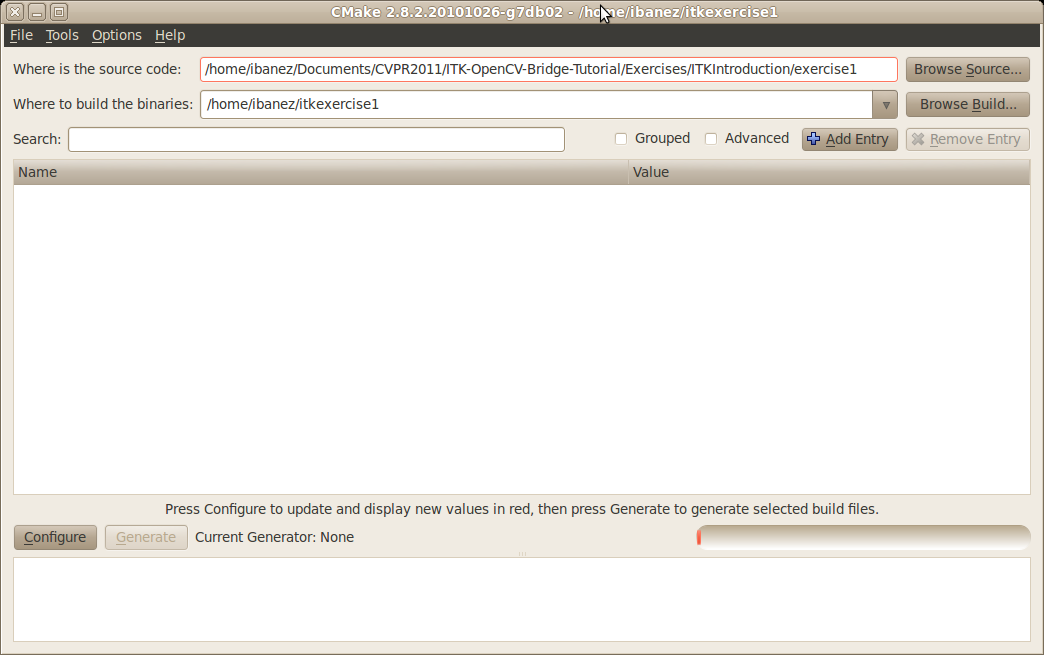
\includegraphics[width=0.5\paperwidth]{Screenshot-CMakeGUI-01.png}
\end{center}
\end{frame}

\begin{frame}[fragile]
\frametitle{How to Configure and Build}
\framesubtitle{cmake-gui}
\begin{itemize}
\item Set ``Source Directory'' (where the source code is)
\item Set ``Binary Directory'' (where to build the executable)
\item Click on ``Configure''
\end{itemize}
\begin{center}
  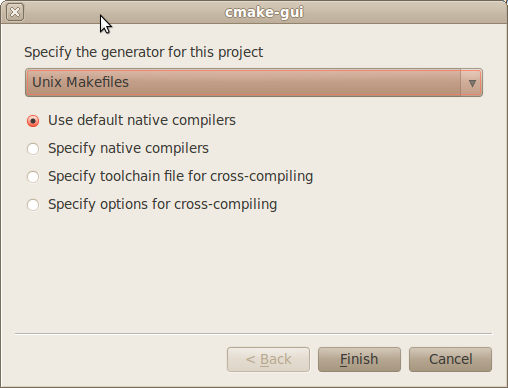
\includegraphics[width=0.7\paperwidth]{Screenshot-CMakeGUI-02.png}
\end{center}
\end{frame}

\begin{frame}[fragile]
\frametitle{How to Configure and Build}
\framesubtitle{cmake-gui}
\begin{itemize}
\item You will get an error message
\end{itemize}
\begin{center}
  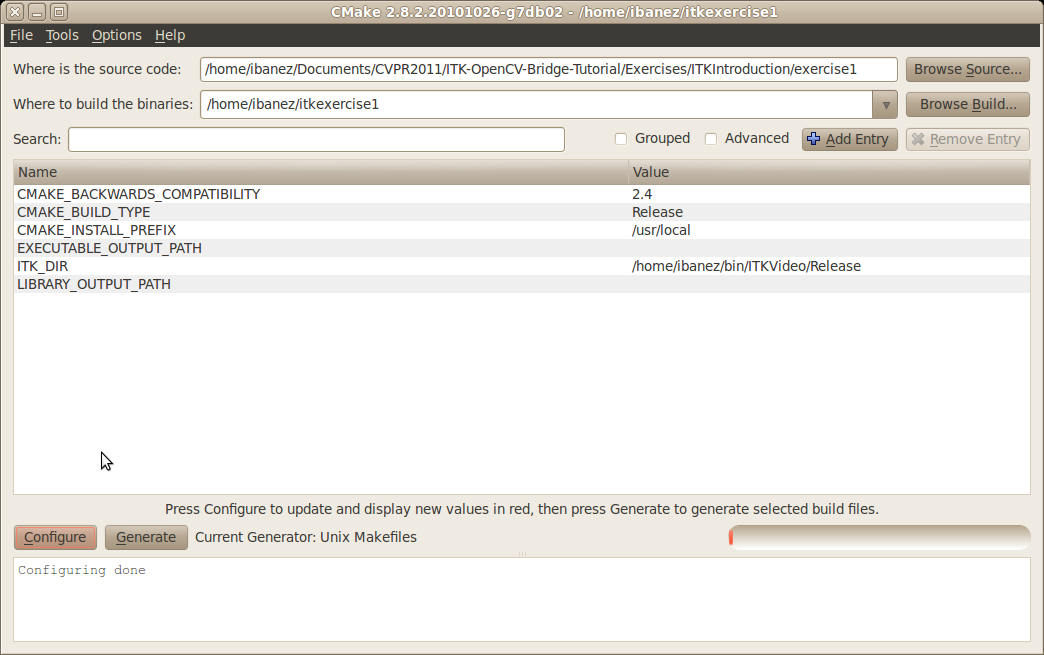
\includegraphics[width=0.3\paperwidth]{Screenshot-CMakeGUI-03.png}
\end{center}
\begin{itemize}
\item Because the project needs ITK and we have not provided it yet
\end{itemize}
\end{frame}


\begin{frame}[fragile]
\frametitle{How to Configure and Build}
\framesubtitle{cmake-gui}
\begin{itemize}
\item Provide the path to ITK in the ITK\_DIR variable
\item /home/tutorial/bin/ITKVideo/Release
\end{itemize}
\begin{center}
  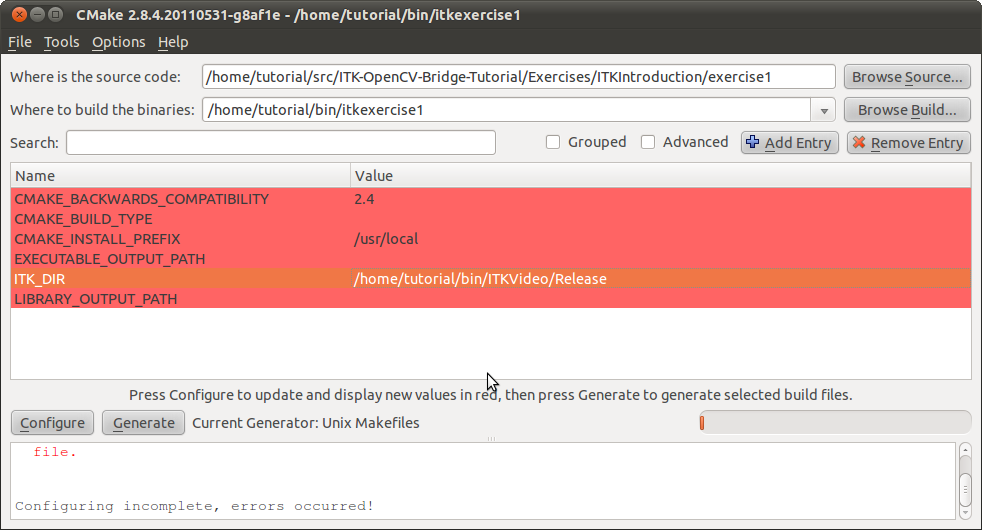
\includegraphics[width=0.7\paperwidth]{Screenshot-CMakeGUI-04.png}
\end{center}
\end{frame}

\begin{frame}[fragile]
\frametitle{How to Configure and Build}
\framesubtitle{cmake-gui}
\begin{itemize}
\item Click on ``Configure''
\item Click on ``Generate''
\end{itemize}
\begin{center}
  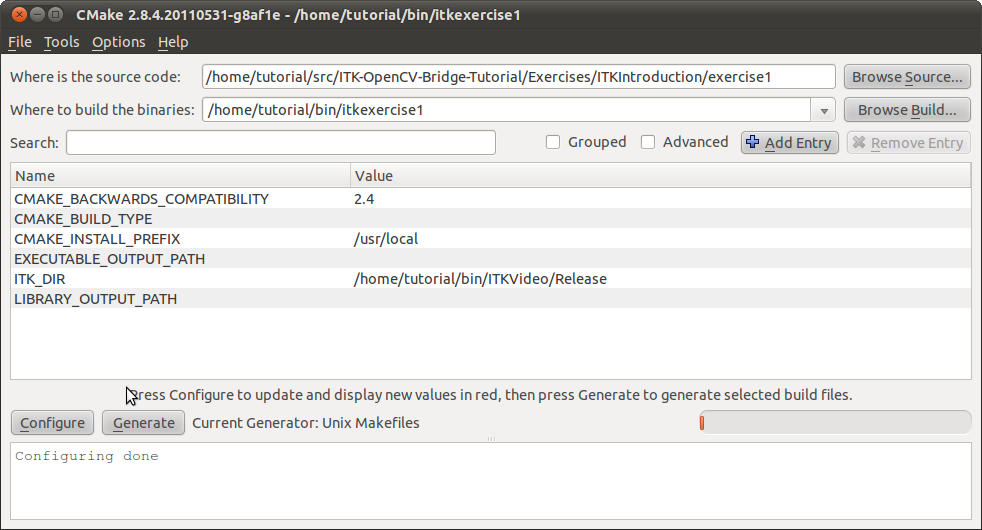
\includegraphics[width=0.7\paperwidth]{Screenshot-CMakeGUI-05.png}
\end{center}
\end{frame}

\begin{frame}[fragile]
\frametitle{How to Build}
\framesubtitle{make}
\begin{itemize}
\item In the command line do:
\begin{verbatim}
cd  /home/tutorial/bin/itkexercise1
make
\end{verbatim}
\end{itemize}
\end{frame}

\begin{frame}[fragile]
\frametitle{How to Run}
\framesubtitle{/home/tutorial/bin/itkexercise1}
\begin{itemize}
\item While in the binary directory:
\begin{verbatim}
/home/tutorial/bin/itkexercise1
\end{verbatim}
\item In the command line type:
\begin{verbatim}
./BasicImageFilteringITK          \
      ~/data/baboongray.png       \
      ./baboongrayMedian.png      \
      3  3
\end{verbatim}
\end{itemize}
\end{frame}

\begin{frame}[fragile]
\frametitle{How to View the Result}
\framesubtitle{Image viewing application ``eye of gnome'': eog}
\begin{itemize}
\item In the command line type:
\begin{verbatim}
eog ~/data/baboongray.jpg &
eog ./baboongrayMedian.png &
\end{verbatim}
\end{itemize}
\end{frame}

\begin{frame}[fragile]
\frametitle{Result of Median Filter}
\begin{center}
  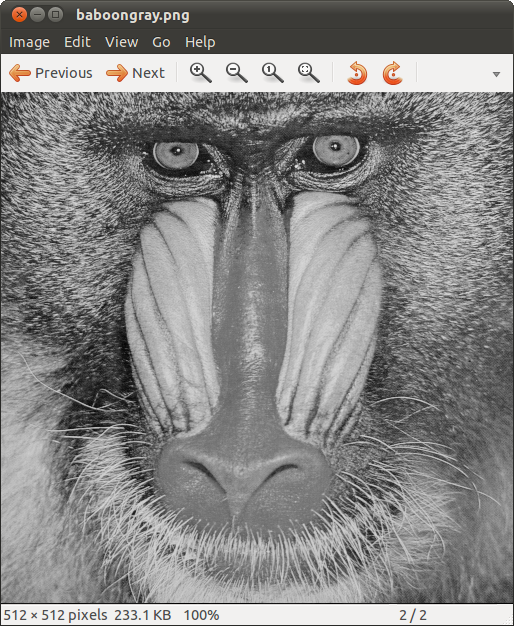
\includegraphics[width=0.45\paperwidth]{Screenshot-baboongray-01.png}
  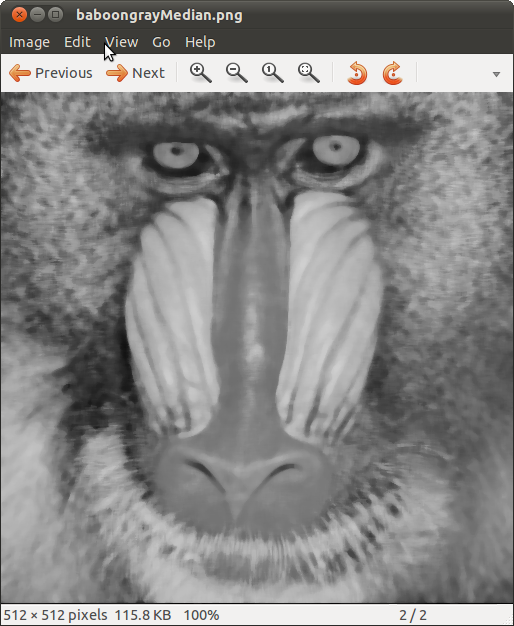
\includegraphics[width=0.45\paperwidth]{Screenshot-baboongrayMedian-01.png}
\end{center}
\end{frame}

\begin{frame}[fragile]
\frametitle{Excercise 1}
\framesubtitle{Replace the filter with another one}
\begin{itemize}
\item Select a Filter from the Doxygen documentation\\
(e.g. MeanImageFilter)
\item Replace the MedianImageFilter with the selected filter
\item Recompile
\item Rerun
\end{itemize}
\end{frame}

\begin{frame}
\frametitle{Excercise 1}
\framesubtitle{ITKIntroduction/exercise1/BasicImageFilteringITKAnswer1.cxx}
\begin{itemize}
\item First we replace the Header file:
\lstlistingwithnumber{21}{21}{BasicImageFilteringITKAnswer1.cxx}
\end{itemize}
\begin{itemize}
\item Then we replace the Filter instantiation:
\lstlistingwithnumber{49}{49}{BasicImageFilteringITKAnswer1.cxx}
\end{itemize}
\end{frame}

\begin{frame}[fragile]
\frametitle{How to Build}
\framesubtitle{make}
\begin{itemize}
\item In the command line do:
\begin{verbatim}
cd  /home/tutorial/bin/itkexercise1
make
\end{verbatim}
\end{itemize}
\end{frame}

\begin{frame}[fragile]
\frametitle{How to Run}
\framesubtitle{/home/tutorial/bin/itkexercise1}
\begin{itemize}
\item While in the binary directory:
\begin{verbatim}
/home/tutorial/bin/itkexercise1
\end{verbatim}
\item In the command line type:
\begin{verbatim}
./BasicImageFilteringITK        \
      ~/data/baboongray.png     \
      ./baboongrayMean.png      \
      3  3
\end{verbatim}
\end{itemize}
\end{frame}

\begin{frame}[fragile]
\frametitle{How to View the Result}
\framesubtitle{Image viewing application ``eye of gnome'': eog}
\begin{itemize}
\item In the command line type:
\begin{verbatim}
eog ~/data/baboongray.jpg &
eog ./baboongrayMean.png &
\end{verbatim}
\end{itemize}
\end{frame}

\begin{frame}[fragile]
\frametitle{Result of Mean Filter}
\begin{center}
  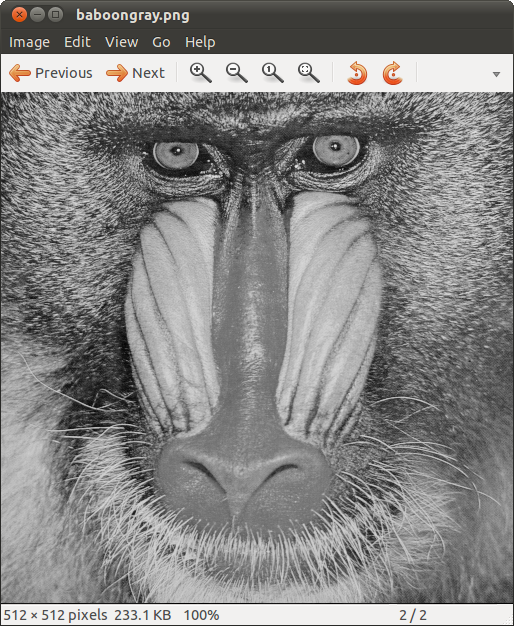
\includegraphics[width=0.45\paperwidth]{Screenshot-baboongray-01.png}
  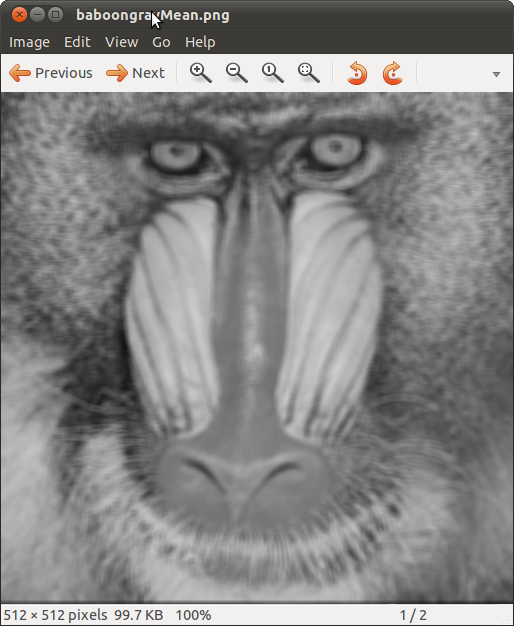
\includegraphics[width=0.45\paperwidth]{Screenshot-baboongrayMean-01.png}
\end{center}
\end{frame}

\begin{frame}[fragile]
\frametitle{Find All Other Exercises}
\begin{itemize}
\item Go to the binary directory
\begin{verbatim}
cd ~/bin/ITK-OpenCV-Bridge-Tutorial/Exercises
\end{verbatim}
\end{itemize}
\end{frame}

\begin{frame}
\frametitle{Basic Filtering - Canny Filter}
\framesubtitle{ITKIntroduction/exercise1/BasicImageFilteringITKAnswer2.cxx}
\lstlistingwithnumber{21}{23}{BasicImageFilteringITKAnswer2.cxx}
\end{frame}

